\documentclass[a4paper,12pt]{article}


% Set margins
\usepackage[hmargin=2cm, vmargin=2cm]{geometry}
\usepackage{setspace}
\onehalfspacing



% Language packages
\usepackage[utf8]{inputenc}
\usepackage[T1]{fontenc}
\usepackage[magyar]{babel}

% AMS
\usepackage{amssymb,amsmath}

% Graphic packages
\usepackage{graphicx}
\graphicspath{ {./kepek/} }

% Colors
\usepackage{color}
\usepackage[usenames,dvipsnames]{xcolor}

\usepackage{hyperref}
\hypersetup{
    linkcolor=blue,
    filecolor=magenta,      
    urlcolor=cyan,
}

% Code style
 
\usepackage{listings}
\usepackage{xcolor}
 
\definecolor{codegreen}{RGB}{17, 209, 94}
\definecolor{codegray}{RGB}{74, 74, 74}
\definecolor{codeblue}{RGB}{0, 146, 209}
\definecolor{backcolour}{RGB}{242, 242, 242}
 
\lstdefinestyle{mystyle}{
    backgroundcolor=\color{backcolour},   
    commentstyle=\color{codegreen},
    keywordstyle=\color{codeblue},
    numberstyle=\tiny\color{codegray},
    stringstyle=\color{codeblue},
    basicstyle=\ttfamily\footnotesize,
    breakatwhitespace=false,         
    breaklines=true,                 
    captionpos=b,                    
    keepspaces=true,                 
    numbers=left,                    
    numbersep=5pt,                  
    showspaces=false,                
    showstringspaces=false,
    showtabs=false,                  
    tabsize=2
}


 
\lstset{style=mystyle}


% Enumeration
\usepackage{enumitem}



\begin{document}

\begin{center}
	\Large \textbf{MISKOLCI EGYETEM}
	\\
	\Large \textbf{GÉPÉSZMÉRNÖKI ÉS INFORMATIKAI KAR}
	\vskip 1cm
	\begin{figure}[h]
		\centering
		
\includegraphics[width=0.3\textwidth]{logo}
	\end{figure}
	\\  
	\Large \textbf{Alkalmazott Informatikai Intézeti Tanszék}
	\vskip 1cm
	\huge \textbf{Blokkon levő adatok automatikus feldolgozása}
	\vskip 1cm
	\Large \textbf{Szakmai gyakorlat (GEIAKSzGyBI{\_}TM-B)}
	\vskip 1cm
	\huge \textbf{Szabó Szilveszter Rafael}
	\\
	\LARGE \textbf{YTBR1C}
	\vskip 1cm
	\Large \textbf{Konzulens: Piller Imre}

\end{center}

\newpage
\tableofcontents

\newpage 
\section{Munkanapló}
\begin{figure}[h]
	\centering
	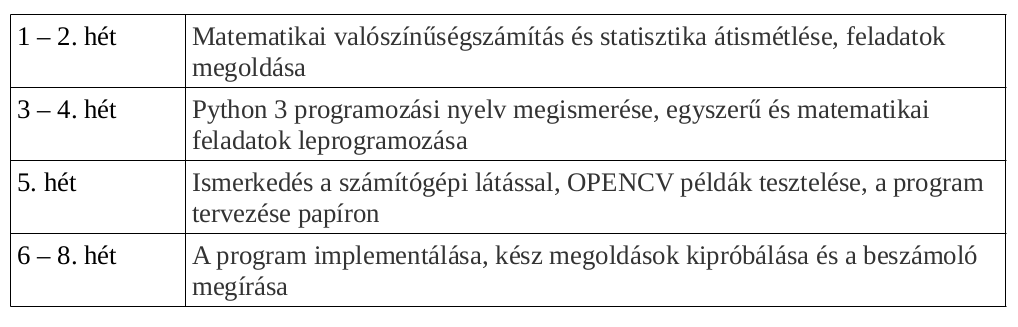
\includegraphics[width=16cm]{munka}
	
\end{figure}

\newpage
\section{Bevezetés}
Mérnökinformatikus alapszak során 8 hetes szakmai gyakorlat elvégzésére van szükség, hogy  oklevelet szerezhessek. Mielőtt még beindult a tavaszi félév, már sok helyen nézelődtem gyakornoki programok között, hogy hova is mehetnék majd nyáron, de nem találtam olyan céget, ahol eltudtam volna helyezkedni, mert még nem volt megfelelő tudásom hozzá. Így végül úgy döntöttem, hogy szakmai gyakorlatomat a Miskolci Egyetemen végzem el. Azért választottam ezt a lehetőséget, mert így nagyon sokat tudtam tanulni, viszonylag rövid idő alatt és azon a területen amivel majd későbbiekben is foglalkozni szeretnék. 
 
Az egyetem Alkalmazott Matematikai Intézeti Tanszék-én töltöttem Piller Imre vezetésével, aki végig nagy segítségemre volt a szakmai gyakorlat alatt. A hetek alatt nagyrészben a számítógépes látással foglalkoztam. Saját feladatot találtam ki magamnak, egy olyan szoftvert ami a bolti nyugtákon levő adatokat elemzi ki és egy adatbázisban tárolja azokat. Az első hetekben beleástam magam a Python programozási nyelvbe és mellette párhuzamosan a matematikai valószínűségszámításba és statisztikába. Az alapozást követő hetekben pedig a szoftverrel foglakoztam. A programomban különböző feldolgozási lépéseken esnek át a fotók, melyek a vágás, a zajszűrés, szerkezeti elemzések(szegmentáció), optikai karakter felismerés, szöveges adatok utófeldolgozása és azok adatbázisban való tárolása. Ennek a projektnek köszönhetően sikerült egy manapság igen fejlődő részét megismernem az informatikának. 

\newpage
\section{Programról röviden}

A fejlesztés során törekedtem, hogy minél több technológiát, eszközt megismerjek ami a segítségemre lehet a későbbiekben. Az egész nyílt forráskódú projektekre épül. Ubuntu 18.04 LTS operációs rendszert használtam mindvégig, amely ilyen jellegű programozásnál egyszerűbb fejlesztést biztosított számomra. A szoftver Python 3 programozási nyelven íródott és a következő programozói könyvtárakat, eszközöket használtam hozzá: 

\begin{itemize}
	\item OpenCV
	\item Numpy
	\item Matplotlib	
	\item Flask	
\end{itemize}

Az OpenCV, ahogy nevéből is adódik (Open Source Computer Vision Library) egy nyílt forráskódú számítógépi látással (és gépi tanulással) foglalkozó programozói könyvtár, melyet azért írtak, hogy egységes környezetet biztosítson a gépi látással foglalkozó programoknak. 2500-nál is több optimizált algoritmus található benne melyek egészen széles alkalmazási terület lefednek, párat ebből kiemelve ami számomra is fontos szerepet játszik, ilyen például az objektum felismerés, a  képi szegmentáció és felismerés.

A NumPy egy olyan csomag Python-hoz mely nélkülözhetetlen a tudományos számításokhoz, nagy többdimenziós tömbök és mátrixok használatát támogatja egy nagy magas szintű matematikai függvénykönvytárral.

A Matplotlib egy kiegészítő könyvtár, melynek segítségével 2D-s ábrázolásokat készíthetünk (függvények, kép megjelenítés) sokféleképpen. 

Fejlesztés során Jupyter Notebook-ot használtam még, mely lényegében olyan mint egy munkafüzet. Webes felületen lehet benne szerkeszteni programjainkat, dokumentációkat. Egységekre tudjuk bontani a programkódunkat, az egyszerűbb megértés érdekében mely nagy segítséget jelent a program írása/tesztelése közben

A programkód jelenleg tesztelési fázisban van, csak lokális gépen fut. Sok finomhangoláson kell még átesni, hogy legalább 90\% -os működést biztosítson, mert a blokkok általában gyűröttek, megvannak szakadva itt-ott, hiányos a nyomtatás. Sok tényezőre kell odafigyelni, és későbbiekben betanítani az algoritmust  ezekre az esetekre. A programom teljes körű webes applikációnak készül amihez, majd Flask webes keretrendszert fogom használni. 

\newpage
\section{Vágási folyamatok}
A programom több részből áll, melyeket részletesen bemutatok programkóddal illetve képekkel az alábbi bekezdésekben. Először az alapvető könyvtárakat mutatom be és módosításokat a mintaképen. Ezután meghatározom a blokk kontúrját, majd abból 4 pontot amely a vágáshoz szükséges. A 4 pont meghatározása, rendszerezése után kiszámolom a blokk hosszát és szélességét, majd megtörténik a vágás, a transzformációk, és a küszöbölés. Az így kapott képen a későbbiekben elvégzek bizonyos szegmentációt, majd optikai karakterfelismerést azon a területen, majd ezt az információt adatbázisban tárolom. 

\subsection{Könyvtárak importálása}
Legelőször beimportáltam a megfelelő könyvtárakat. Matplotlib-et csak tesztelési célok miatt használtam, hogy lássam az eredményt Jupyter Notebook-ban. 
\begin{lstlisting}[language=Python, caption=Könvytárak importálása]
from matplotlib import pyplot as plt
import numpy as np
import cv2 as cv
\end{lstlisting}



\subsection{Alapvető módosítások}
A következő részben beolvastam a mintaképet, melyről készítettem egy másolatot, hogy majd visszatudjam később számolni az eredeti méretre vonatkozó szélességi és hosszúsági értékeket. Ezt azért tettem, mert a képet át kell méreteznem kisebbre a gyorsabb futás és jó eredmény eléréséhez. A megfelelő hosszúsági értéket 500px-nél határoztam meg, így igen hatékonyan lehet akár több tucat képpel is dolgozni egyszerre. A shape() függvénynel lekérdezhetjük a kép szélességét, hosszát egyaránt. Először kiszámoltom a kép arányát, az adott hossz és az eredeti hossz értékekből, majd meghívtam a resize() függvényt a kódban látható paraméterekkel.
\begin{figure}[h]
	\centering
	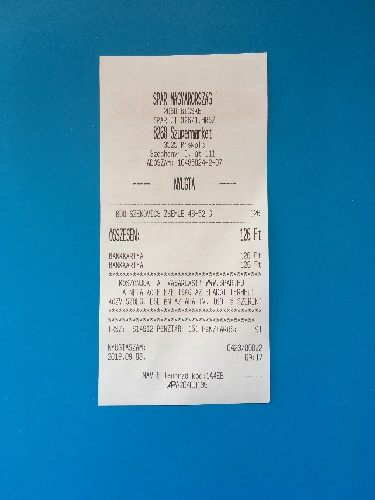
\includegraphics[width=5cm]{1d_resized}
	\caption{Átmérezett kép}
\end{figure}
\\Ahhoz, hogy éleket tudjunk detektálni, először szükséges a képet fekete-fehérré alakítani. Ezután meghívjuk a GaussianBlur() függvényt amellyel elhomályosítjuk a képet, hogy könnyebben eltudjuk szeparálni a blokkot a háttértől. 
\begin{figure}[h]
	\centering
	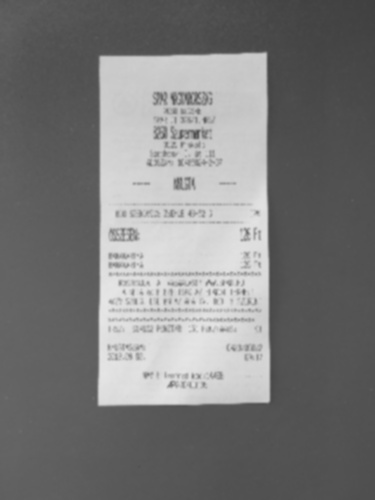
\includegraphics[width=5cm]{3d_blur}
	\caption{Fekete-fehér elhomályosított kép}
\end{figure}
\\Ezután az elhomályosított képre alkalmazzuk a Canny() függvényt, melyben paraméterként két határértéket adunk meg a küszöbölésre. Így egész jó élkiemelést kapunk a blokkra nézve. 
\begin{figure}[h]
	\centering
	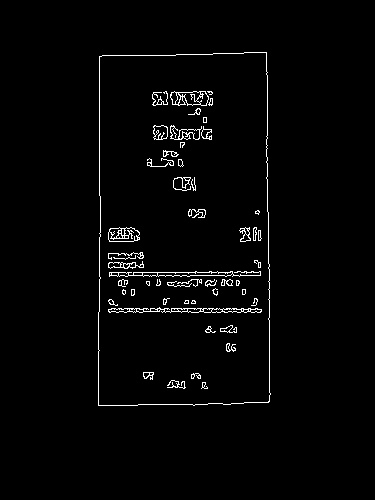
\includegraphics[width=5cm]{4d_cannyedged}
	\caption{Detektált élek Canny() függvénnyel}
\end{figure}
\begin{lstlisting}[language=Python, caption=Alapvető műveletek elvégzése]
image = cv.imread("test.jpg")

original = image.copy()blurred = blur.copy()

height = 500
ratio = height / image.shape[0]
image = cv.resize(image,(int(ratio * image.shape[1]), height))

grayscale = cv.cvtColor(image, cv.COLOR_BGR2GRAY)

blur = cv.GaussianBlur(grayscale, (5, 5), 0)

edge = cv.Canny(blur, 75, 250)
\end{lstlisting}

\subsection{Kontúr meghatározása}

Most, hogy már megvannak a detektált élek, meg kell határoznunk a kontúrt. A findContours() függvénnyel történik a meghatározása, melyben paraméterként átadjuk a éldetektált képet, a visszatérési értékeket lista típusúra állítjuk, a kontúr közelítés módját CHAIN{\_}APPROX{\_}SIMPLE algoritmussal végezzük, amely csak a szükséges végpontokat választja ki, a fölöslegesek eltávolítja, így könnyen megkapjuk majd a 4 pontból álló téglalapot. Következő lépésben a legnagyobb kontúrt kell kiválasztanunk, ezért csökkenő sorrendben rendezzük, hogy minél hamarabb megtaláljuk. Ezután van egy for ciklusunk amelyben először az arcLenght() függvény kerül meghívásra. Ez lényegében zárt kerületű négyzetet(téglalapot) keres a képen, és az approxPolyDP() függvény segítségével becsüljük meg a téglalapot. Ha az approx értéke 4 akkor megvan a téglalapunk illetve négyzetünk. A drawContours()-al kirajzolom az átméretezett képre a téglalapot.

\begin{figure}[h]
	\centering
	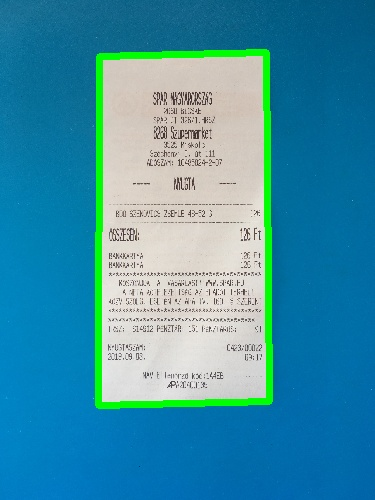
\includegraphics[width=5cm]{5d_squared}
	\caption{A megtalált kontúrvonal}
\end{figure}


\begin{lstlisting}[language=Python, caption=Kontúr kiszámolása és megjelenítése]
contours = cv.findContours(edge.copy(),cv.RETR_LIST,cv.CHAIN_APPROX_SIMPLE)
contours = contours[1]
contours = sorted(contours, key=cv.contourArea, reverse=True)
for c in contours:
    perimeter = cv.arcLength(c, True) 
    approx = cv.approxPolyDP(c,0.02*perimeter,True) 
    if len(approx) == 4:
        square = approx
        break

squared = cv.drawContours(image, [square], -1, (0, 255, 0), 5)
\end{lstlisting}

\subsection{4 pont kinyerése}
A kontúr meghatározásánál, már megkaptuk a 4 pontot, de szükségünk van kisebb módosításokra, hogy egyértelmű legyen. Először is a reshape() függvénnyel "megformázzuk" a points tömbünket, mert tömb a tömben határozodótt meg (az alábbi képen szemléltetem). 
\begin{figure}[h]
	\centering
	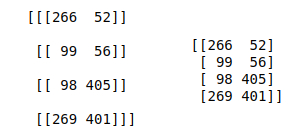
\includegraphics[width=5cm]{matrix}
	\caption{Kapott és formázott mátrix}
\end{figure}
\\Egy új 4x2-es mátrixban fogom tárolni a 4 pont hosszúsági és szélességi koordinátáit, melyet az óramutató járásával megegyezően rendszerezek. Így elindulva a bal felső sarokból jobbra bejárjuk a pontokat és megkapjuk a téglalap 4 pontját. Majd ezt a for ciklus segítségével megjelölöm a képen.
\begin{figure}[h]
	\centering
	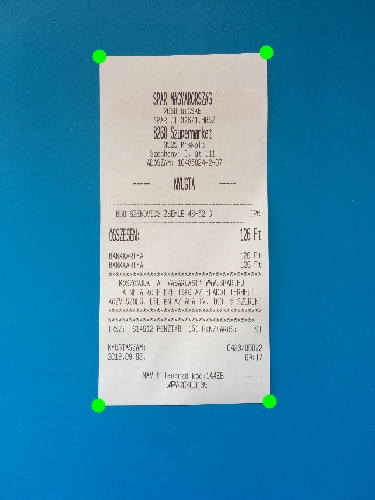
\includegraphics[width=5cm]{6d_pointed}
	\caption{4 pont megjelenítése a képen}
\end{figure}

\begin{lstlisting}[language=Python, caption=A 4 pont rendszerezése]
points = square.reshape(4, 2)
rect = np.zeros((4, 2), dtype = "float32")

summas = points.sum(axis = 1)

rect[0] = points[np.argmin(summas)]  #Top-left
rect[2] = points[np.argmax(summas)]  #Bottom-right

diff = np.diff(points, axis = 1)
rect[1] = points[np.argmin(diff)]   #Top-right
rect[3] = points[np.argmax(diff)]   #Bottom-left
for i,j in rect:
    cv.circle(pointed,(i,j), 7, (0,255,0), -1)
\end{lstlisting}

\subsection{Végső műveletek elvégzése}

Mivel átméretezett képpel dolgoztam eddig, szükséges a mátrix értékeinek visszaszámolása az eredeti méretnek megfelelően, ezt a program elején meghatározott arány segítségével oldottam meg. Ezután minden egyes koordinátát különszedtem. A következő sorokban mind az alsó, felső, bal illetve jobb oldali pontok közötti távolságokat kiszámítom és ebből a maximumot választom, mert így biztosan nem veszítünk el információt a blokkról. Ezután létrehozok egy output mátrixot, melyben megadom az előbb kiszámított értékeket az óramutatójárásával és x illetve y koordináták szerint, amiből megkapom a teljes méretű vágott blokott. Ezután elvégzek rajta egy transzformációt és nyújtást.
\begin{figure}[h]
	\centering
	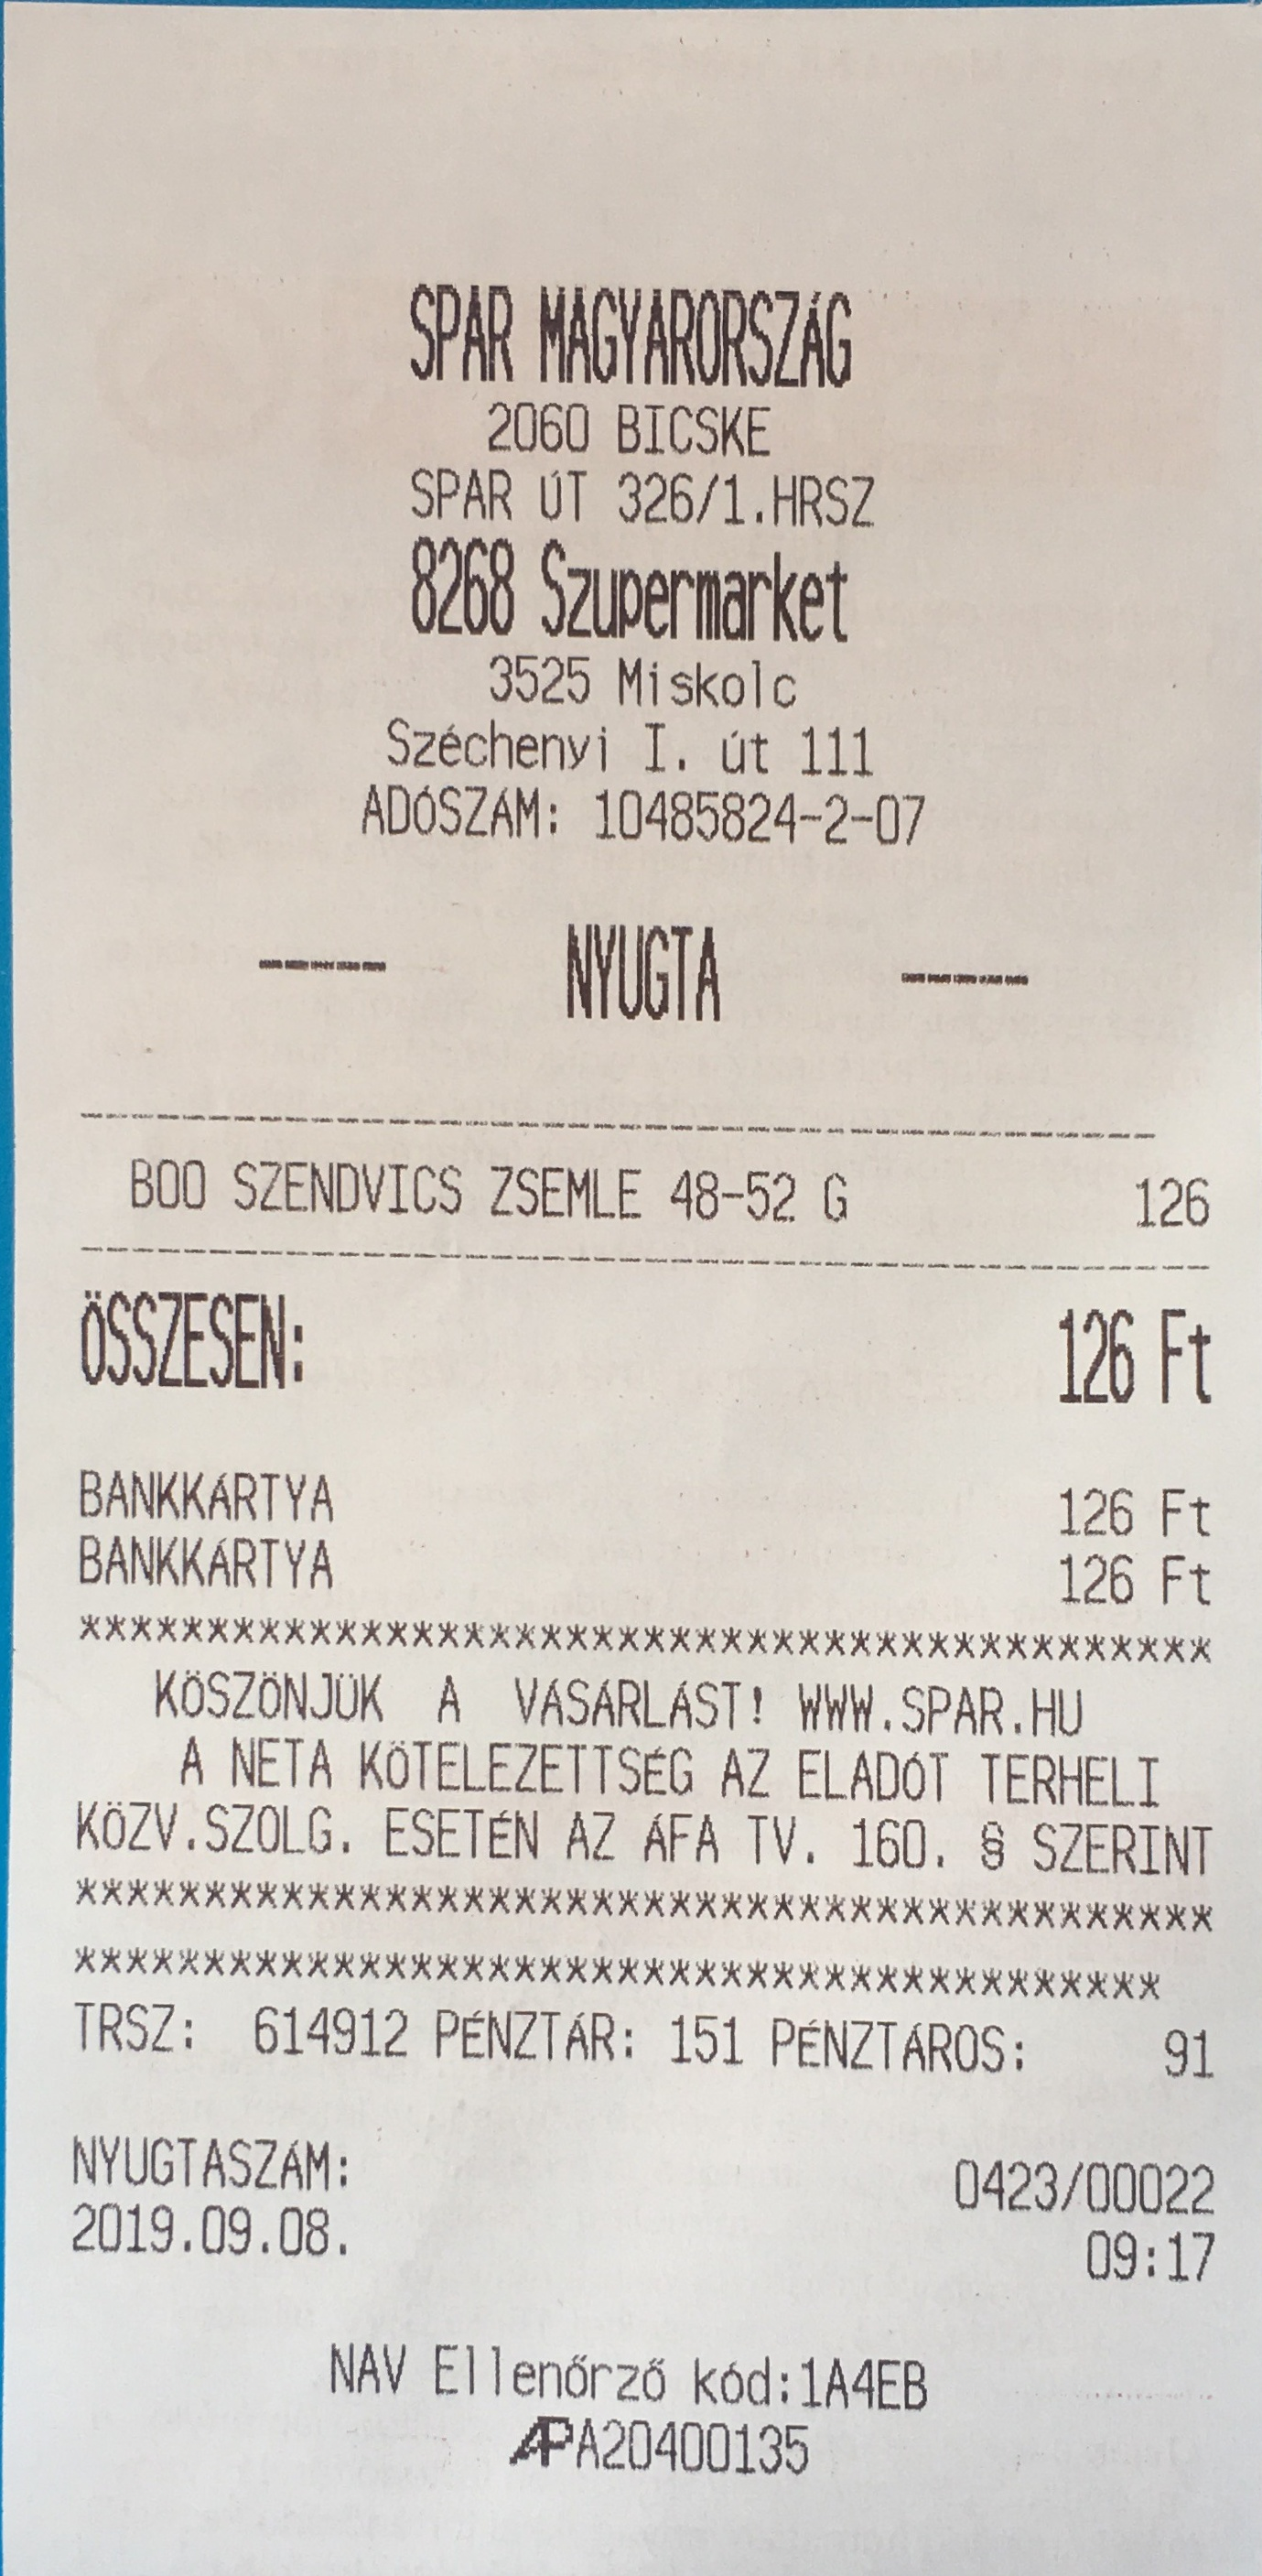
\includegraphics[width=4cm]{7d_warped}
	\caption{A vágott és transzformált kép}
\end{figure}
\\Ez a kép még nem elég tiszta. Olyan hatást akarok elérni, mely ugyanúgy néz ki mintha beolvasnék egy képet lapolvasóval fekete-fehérben, ezért még egy küszöbölést elvégzek rajta.

\begin{figure}[h]
	\centering
	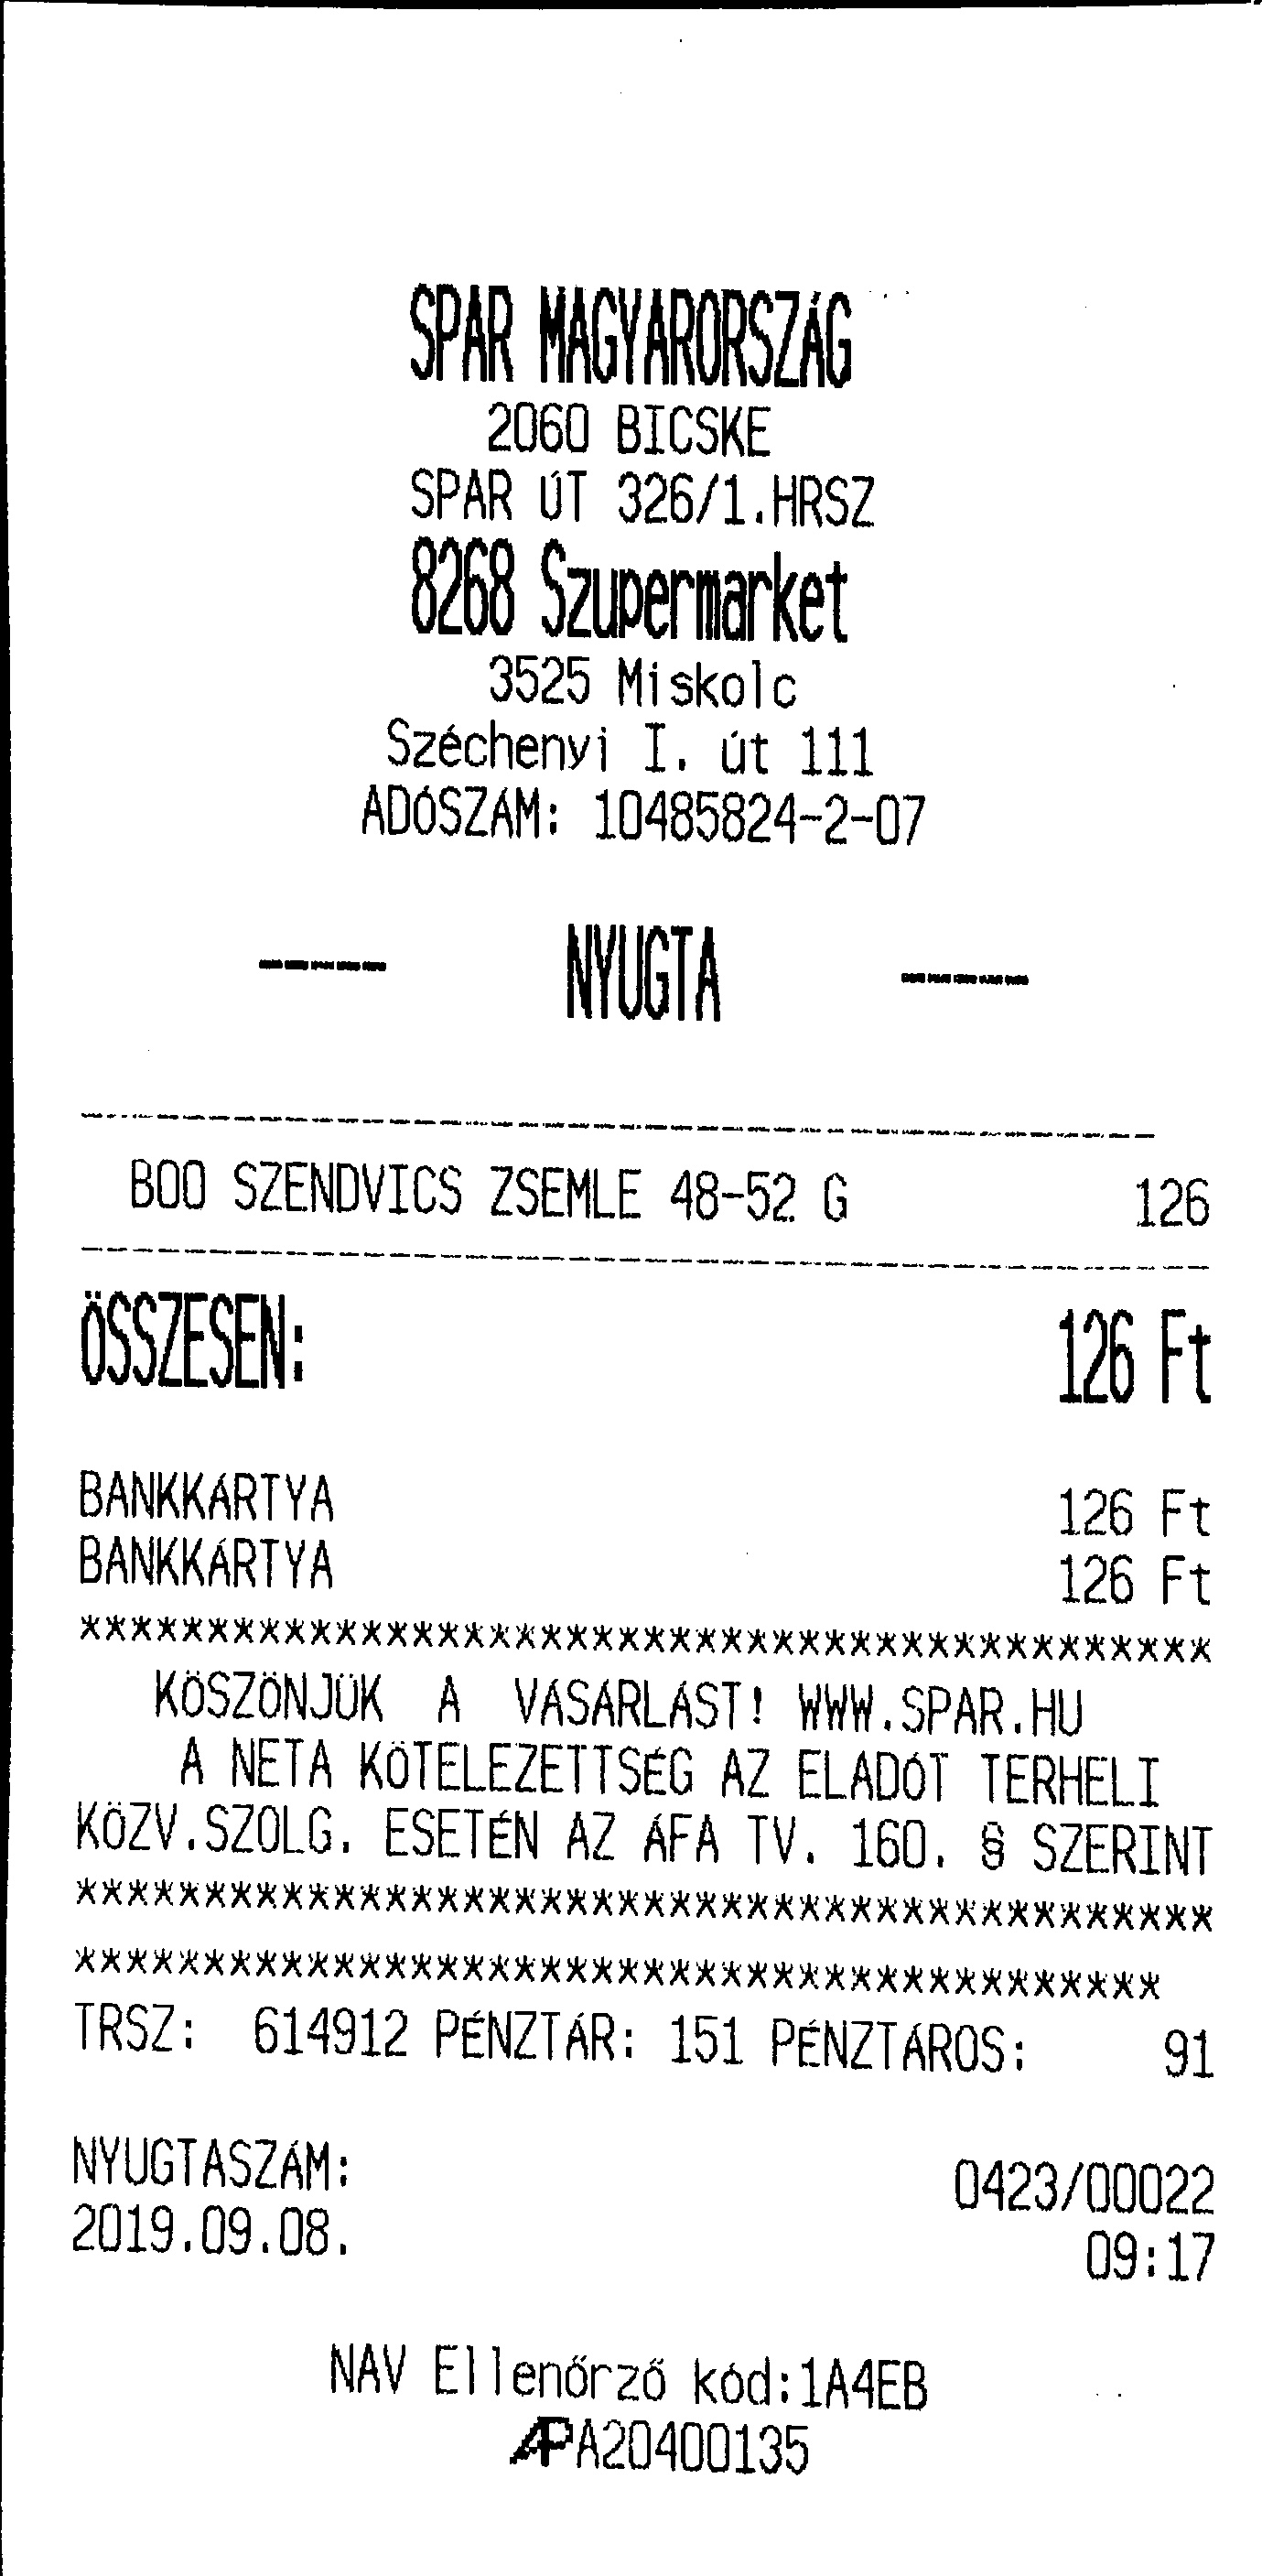
\includegraphics[height=7cm]{8d_final}
	\caption{Küszöböléssel módosított kép}
\end{figure}

\begin{lstlisting}[language=Python, caption= Befejező műveletek]
rect = rect/ratio

(tl, tr, br, bl) = rect

widthTop = np.sqrt(((tr[0]-tl[0])**2) + ((tr[1]-tl[1])**2))
widthBottom = np.sqrt(((br[0]-bl[0])**2) + ((br[1]-bl[1])**2))
maxWidth = max(int(widthTop),int(widthBottom))

heightLeft = np.sqrt(((tl[0]-bl[0])**2) + ((tl[1]-bl[1])**2))
heightRight = np.sqrt(((tr[0]-br[0])**2) + ((tr[1]-br[1])**2))
maxHeight = max(int(heightLeft),int(heightRight))

output = np.array([
    [0,0],
    [maxWidth,0],
    [maxWidth,maxHeight],
    [0,maxHeight]], dtype = "float32")


transform = cv.getPerspectiveTransform(rect, output)
warped = cv.warpPerspective(original, transform, (maxWidth, maxHeight))

bw = cv.cvtColor(warped, cv.COLOR_RGB2GRAY)

ret, thr = cv.threshold(bw,0,255,cv.THRESH_BINARY+cv.THRESH_OTSU)
\end{lstlisting}
A programom jelenleg ennyit tud, amely így lényegében egy blokkolvasó eddig. Most következik majd az érdekesebb rész, ami még nincs teljesen implementálva, ezért csak néhány vázlatot mutatok be a szegmentációról és optikai karakter felismerésről a következő szekciókban.
\newpage
\subsection{Képen levő szövegcsoportok szegmentálása}
Többféle módszer létezik a képen való objektumok, jelen esetben szöveg szegmentálására. Az egyik általában meghatározott környezetben zajlik amelyeket heurisztikus módszerekkel tudunk elérni, ilyen például az az eset amikor a szöveg bekezdésekben van csoportosítva és minden egyes karakter egy egyenes vonalon helyezkedik el. Egy másik módszer a természetes szöveg felismerés, amely egy teljesen más megközelítés, kicsit nehezebb. Ezért volt szükség  azokra a részfeladatokra a programomban, hogy egy tiszta olvasható képet kapjak, mert a lefényképezett natúr képpel nagyon nehezen lehetne dolgozni a bonyolultsága miatt. 2017-ben a Megvii Technology Inc kiadott egy tanulmányt az EAST ( Efficient and Accurate Scene Text) mély tanulás alapú saját szöveg felismerő algoritmusukról. Ez a módszer neurális hálón alapszik, amely direkt arra lett betanítva, hogy felismerje a szövegeket és azok geometriáját képekről. 
\begin{figure}[h]
	\centering
	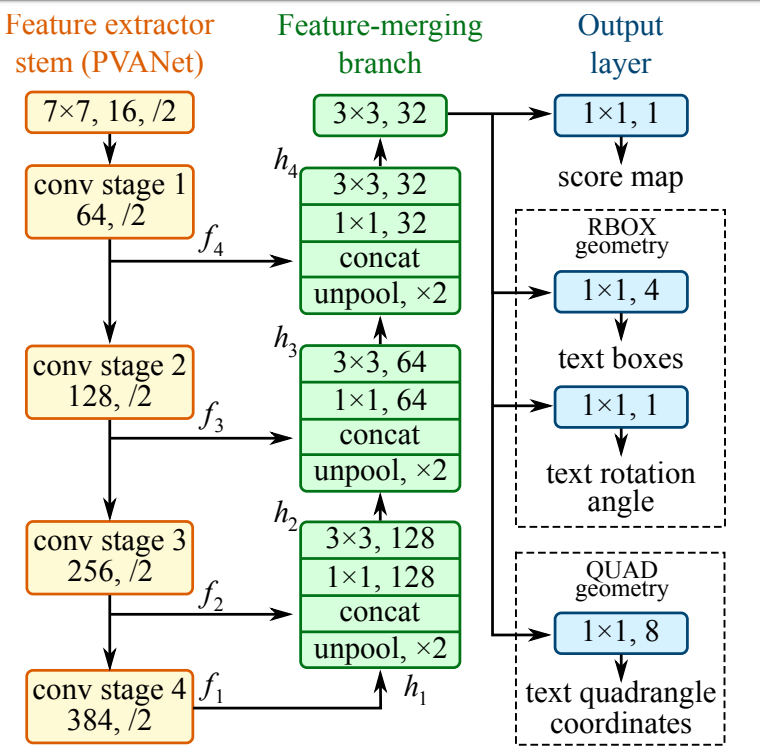
\includegraphics[width=8cm]{east}
	\caption{EAST szöveg felismerő szerkezete (Teljes konvolúciós háló)}
\end{figure}
\\Megtalálható pár implementációja az interneten, viszont ezek nem egészen pontosan dolgoznak. Kifejezetten blokkokra kell majd betanítani, mert a jelenlegi kiadott model a természetes szövegekre van finomhangolva, ilyenek például a közlekedési táblák, hirdető táblák, stb.. Lényegében minden olyan szöveg, amely nagyobb méretben jelenik meg a valóságban, ellentétben a blokkal, ahol sok apró betűből álló szavak találhatók. Alább látható egy implementáció által kapott eredmény.
\newpage
\begin{figure}[h]
	\centering
	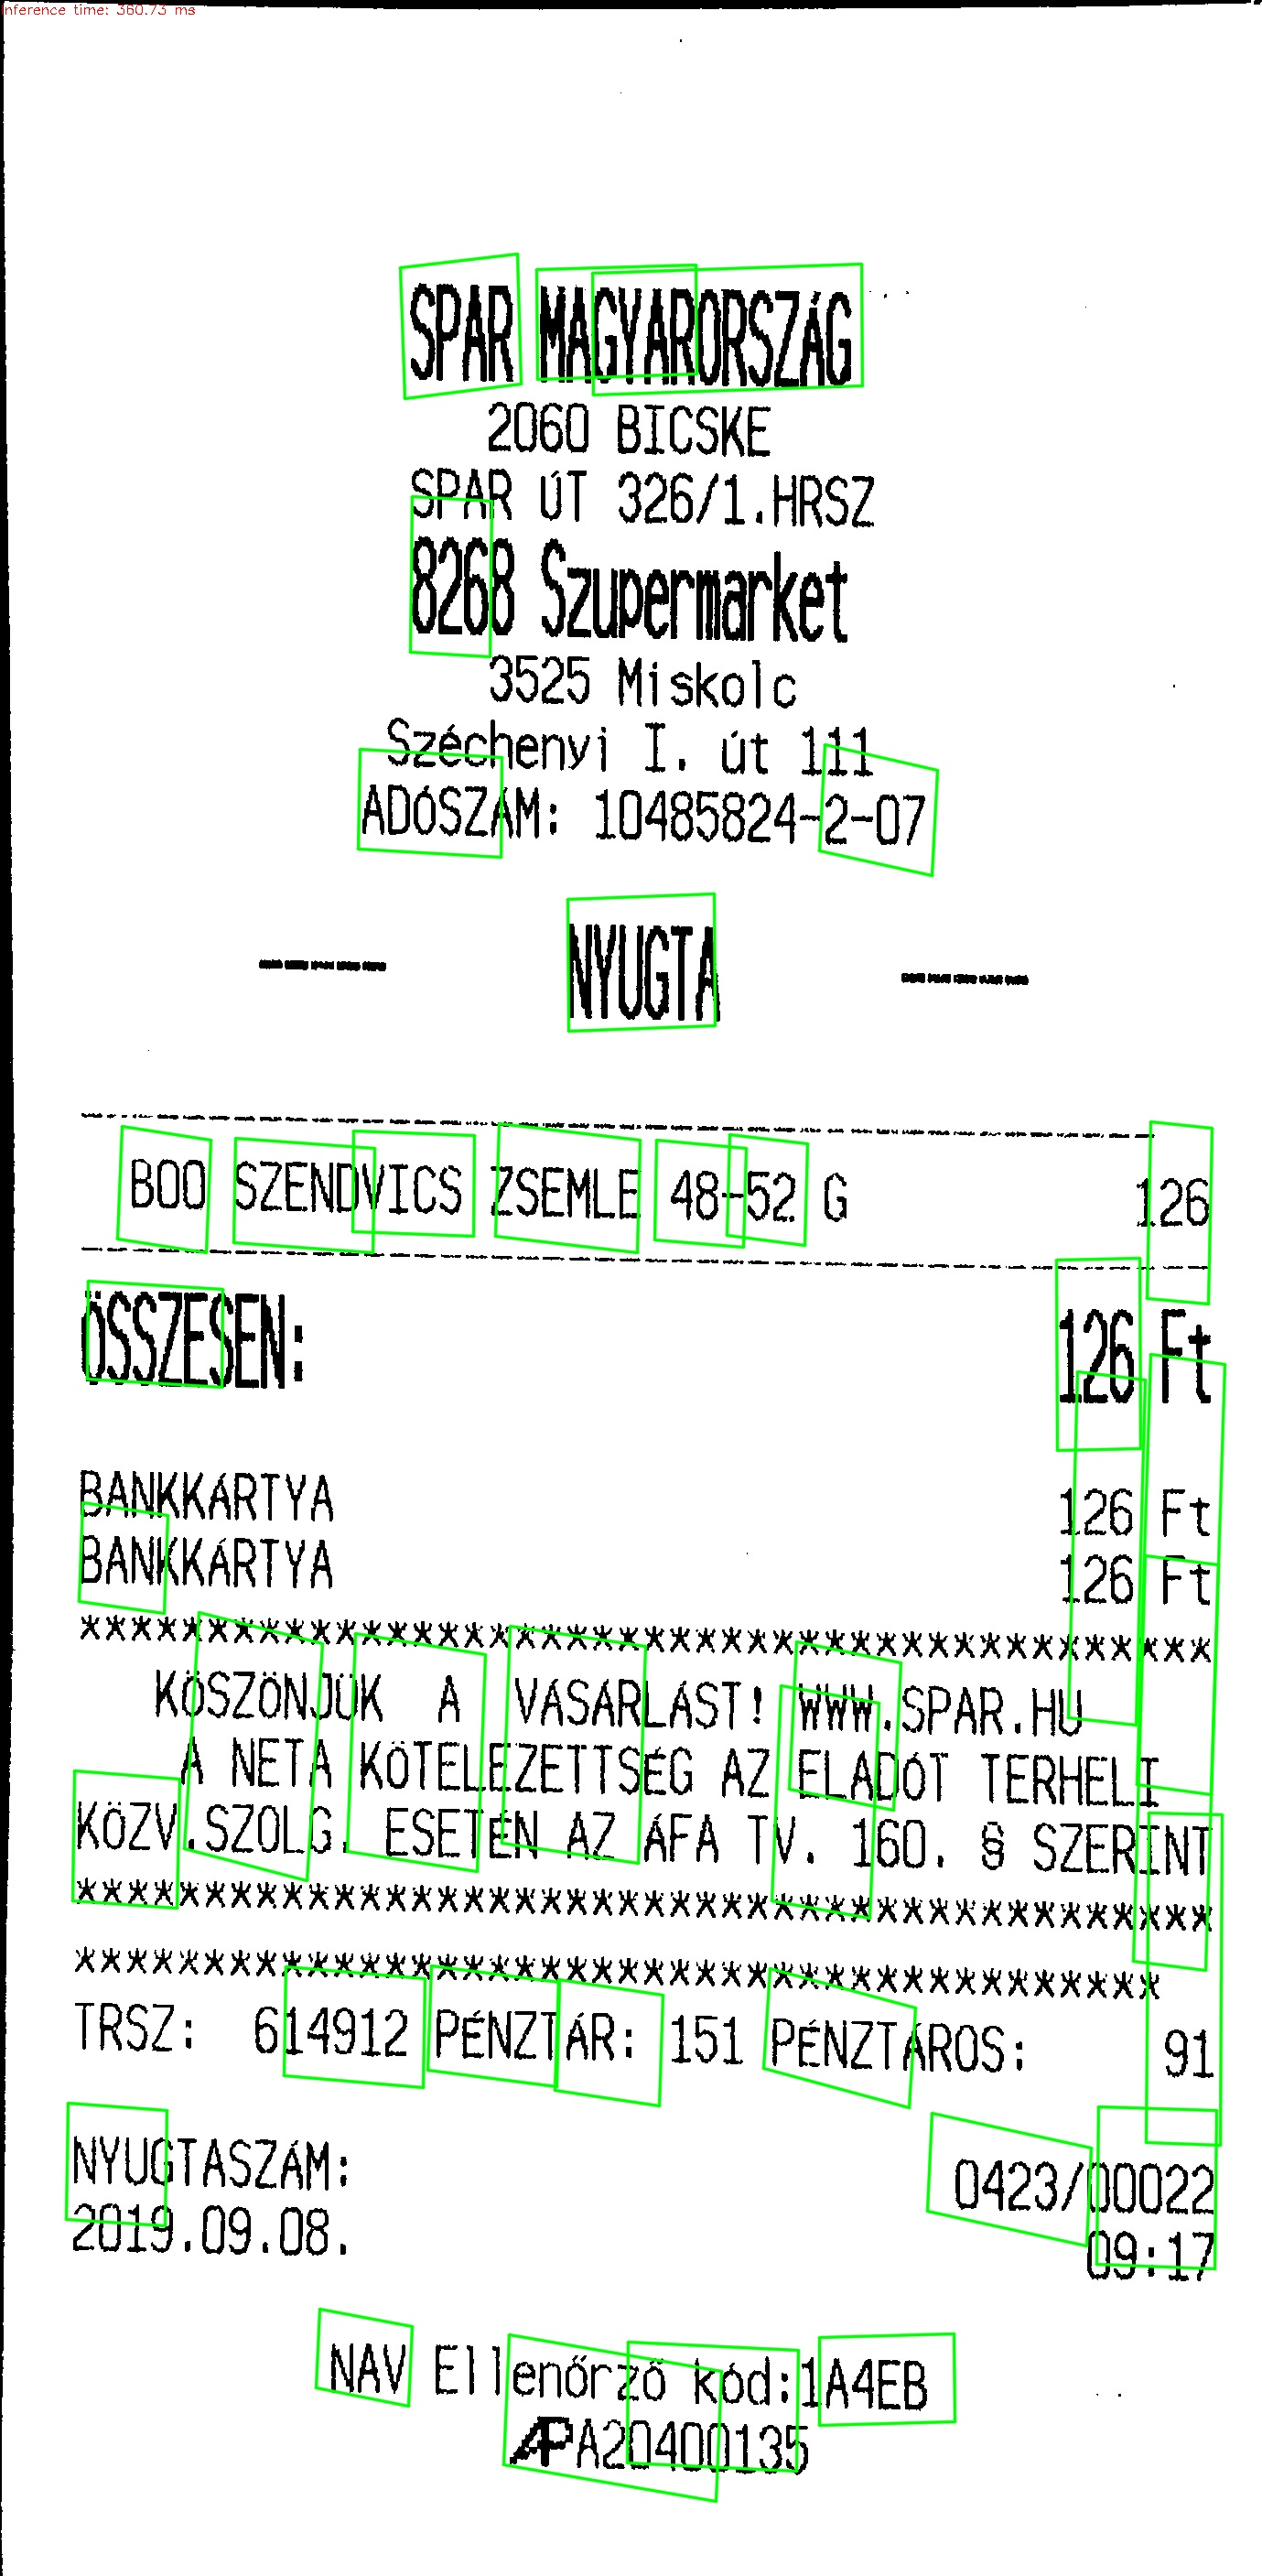
\includegraphics[width=5cm]{out}
	\caption{Szöveg blokkok felismerése EAST szöveg felismerővel}
\end{figure}

A közeljövőben még számos lehetőséget kipróbálok majd, mert még van pár lehetséges megoldás, de egyelőre ez bizonyult a legegyszerűbbnek a teszteléshez. Bővebben a publikációban lehet róla olvasni, hogy hogyan történik a felismerés folyamata. 

\subsection{Távolabbi kilátások: \\Optikai karakterfelismerés és webes applikáció}
Az utolsó előtti rész az optikai karakterfelismerés lesz. A legelterjedtebb és leghatékonyabb eszköz erre a Tesseract nyíltforráskódú szövegfelismerő motor. Ennek segítségével fogom majd a meghatározott szövegblokkokról a szöveget felismerni. 
Amint sikerül kiolvasnom a szöveget, ezt majd tárolni és hozzáférhetővé is kell tennem. Mivel ez egy egyszerű webes applikáció lesz, a Flask keretrendszert fogom használni. Egy egyszerű adatbázist csinálok SQLite segítségével az adatok tárolására. A webes felületen lehet majd elérni a beolvasott adatokat minden egyes blokkról, statisztikákat(hol,mennyiért,mit vásároltunk),stb...
Nagyjából így nézne ki az egész programom működése, amelyre még sok munka vár. Remélem mihamarább elkészül a végleges változat és lehet majd tesztelni éles környezetben is. \

\newpage
\section{Források}
\url{https://www.learnopencv.com/deep-learning-based-text-detection-using-opencv-c-python/}
\\
\url{https://docs.opencv.org/3.4.7/d6/d00/tutorial_py_root.html}
\\
\url{https://arxiv.org/pdf/1704.03155.pdf}


\end{document}
